% \ifdefined\FromMain %
% \else % 
% 	\documentclass[../main.tex]{subfiles}
% 	\let\FromMain\undefined
%   	\begin{document}
% \fi
\documentclass[../main.tex]{subfiles}
\begin{document}

\newpage

\chapter*{Introduction}
 \addcontentsline{toc}{chapter}{\protect\numberline{}Introduction}
\minitoc
\newpage
%\doublespacing %% For correction

\section{Émergence de la microbiologie \textit{in silico}}
La compréhension des mécanismes biologiques inhérents à un micro-organisme ou un écosystème microbien ne passe plus uniquement par des expérimentations à la paillasse mais aussi par des traitements de données et simulations informatiques. Au commencement de la microbiologie, les scientifiques se concentraient sur les maladies infectieuses, affectant à la fois les hommes et les animaux. Le rôle des bactéries dans certaines pathologies, mais aussi dans des processus de bio-transformation comme la fermentation a ensuite commencé à être élucidé. Aujourd’hui, aller plus loin dans l’étude de ces systèmes biologiques implique  la production de données à haut-débit dites \textbf{omiques}. La première d’entre elles, permettant de caractériser le vivant à l'échelle moléculaire, et la plus utilisée est la génomique. Les molécules d’ADN sont séquencées, générant des lectures et motivant le développement d’algorithmes informatiques d'assemblage de ces lectures en contigs. D’autres données omiques portant sur l'analyse des ARN (transcriptomique), des protéines (protéomique) et de la biochimie (métabolomique) ont émergé, accélérant le développement en parallèle de \textbf{modèles informatiques}.  Ces derniers représentent de façon simplifiée un processus ou une réalité ; ils sont construits et alimentés par des données, ici les données omiques, et propose des sorties dont l’objectif est de contribuer à répondre à des questions biologiques.\\

Au-delà de l’étude des bactéries cultivables, la microbiologie s’attelle à étudier des écosystèmes microbiens, aussi appelés microbiotes, composés de plusieurs centaines ou milliers d’espèces différentes. Difficilement contrôlables expérimentalement, composés d’espèces parfois inconnues, ces ensembles sont auditables par la génération de données omiques à haut-débit. Les modèles informatiques sont alors essentiels pour l’intégration de ces données massives et hétérogènes, et surtout pour générer des hypothèses testables sur le fonctionnement des écosystèmes.  Au sein de ces écosystèmes microbiens, il existe des mécanismes complexes d'interactions nécessitant l’analyse du système dans sa globalité et rendant insuffisante l’analyse des membres individuels. Ces interactions ont des effets positifs, négatifs ou neutres sur les organismes qui composent la communauté \citep{Faust2012}. Leur rôle est d’importance et varie selon l'écosystème: protection contre des pathogènes de l'intestin \citep{Zhang2015}, recyclage des matières organiques dans l'écosystème du sol \citep{Hoorman2011, Yadav2018} ou encore, libération de composés d'arômes  \citep{McSweeney2000} responsables de la qualité du vin par exemple \citep{Virdis2021}. Révéler ces interactions en laboratoire est possible en élaborant des co-cultures par paire ou petits groupes d’espèces \citep{Weiss2022} mais devient complexe pour des communautés de grande taille. Ainsi, il existe un réel besoin de créer des modèles informatiques permettant de pallier aux limitations expérimentales et proposer des hypothèses pour expliquer les interactions. \\

En somme, le développement de modèles informatiques pour la microbiologie est motivé par les données omiques, permettant de les analyser, mais également permet de générer de nouvelles hypothèses, testables en laboratoire, pour potentiellement influer sur les systèmes biologiques. Lier les modèles aux données n'est pas un processus trivial, la \textbf{biologie des systèmes} est au c\oe{}ur de ces problématiques.

\section{La biologie des systèmes comme support de l'étude du métabolisme}
La biologie des systèmes associe un organisme à un système et consiste à étudier ce dernier dans son ensemble, et non comme un assemblage de gènes et de protéines ou autres sous-systèmes indivduels \citep{Kitano2002}. La biologie des système englobe en 4 aspects principaux: les données, essentiellement \textit{omiques}, qui constituent la connaissance biologique; la partie \textit{computationelle}, qui construit des modèles informatiques pour effectuer des simulations selon les hypothèses des biologistes et les données disponibles;  l’ \textit{analyse} de ces simulations, permettant de formuler des hypothèses et des prédictions sur le système; et enfin une dimension  \textit{technologique}, qui consiste en les protocoles expérimentaux générant les données initiales mais permettant aussi de vérifier les hypothèses du modèle. Tout comme la microbiologie a évolué vers l'étude des microbiotes, la biologie des systèmes est elle aussi passée à l’échelle de l’écosystème : le système d'étude comprend alors l'ensemble des membres de l'écosystème \citep{osti_5545893}. 

Une question concrète reste l’identification de méthodes pour caractériser les interactions bactériennes dans le cadre posé par la biologie des systèmes. Nous savons que les interactions métaboliques entre bactéries ou avec son hôte consistent en l'échange de molécules impactant ou non le phénotype de l’organisme receveur \citep{Faust2012}. Or, la biologie des systèmes concentre son étude en intégrant plusieurs niveaux que sont les gènes, les protéines ou encore les métabolites. Dans la littérature, un réseau métabolique, qui est une abstraction informatique de l'ensemble des réactions biochimiques pouvant être catalysées par un organisme, c’est-à-dire son \textbf{métabolisme}, a comme concept de base des associations gène-protéine-réaction (GPR) \citep{Thiele.2010}. Ainsi, modéliser le métabolisme à l'aide de réseaux construits à l'échelle du génome (GEMs) répond aux contraintes de la biologie des systèmes et est une piste pour mieux caractériser les communautés bactériennes. A l'échelle d'un organisme, d’une espèce, il existe de nombreuses méthodes informatiques et mathématiques permettant l'analyse métabolique, comme par exemple des analyses numériques basée sur des flux \citep{Orth2010} ou encore sur la topologie des réseaux \citep{kuffner2000}. Si des challenges méthodologiques persistent encore sur la modélisation à l’échelle d’une espèce, ils sont bien plus nombreux à l'échelle de la communauté, qui génère des nouvelles problématiques de modélisation, et de gestion des coûts calculatoires et de la combinatoire des interactions microbiennes possibles.  À ces difficultés s’ajoute la moindre disponibilité de données et la plus faible connaissance biologiques des acteurs individuels en présence. Pourtant, l'étude à haut débit des communautés bactériennes \textit{in silico} est nécessaire pour proposer de nouvelles hypothèses biologiques dans le cercle vertueux de la biologie des système. Cela nécessite le développement de nouvelles méthodes informatiques et mathématiques, discrètes ou numériques, mettant en avant les interactions bactériennes \textit{via} l'étude du métabolisme. 


%
\section{Objectifs de la thèse}

Du point de vue de la modélisation, le défi principal auquel tente de répondre cette thèse est l’identification d'un modèle avec le meilleur compromis entre précision des résultats, versatilité, temps de calcul et pouvoir d’explicabilité. À cette problématique s'ajoute le nombre de mécanismes métaboliques que l'on souhaite modéliser qui augmente avec le nombre d'organismes que le système compte. Ainsi, analyser des communautés naturelles rapidement, avec une parfaite compréhension de l'ensemble du métabolisme de chaque individu au sein de la communauté permettant la prédiction de nouveaux processus d'interaction est utopique et la simplification du système par un modèle pertinent est d’importance. Dans cette thèse, nous avons identifié deux grands formalismes permettant d'analyser des communautés microbiennes et de mettre en avant des interactions. Il existe des méthodes de modélisation numérique du métabolisme apportant la précision requise mais pouvant être limitées par ses besoins en disponibilité des données et connaissance biologique ainsi que par le temps de calcul. Ces limites sont contournées par des approches discrètes, dégradant la précision numérique mais apportant la capacité d'analyser des communautés naturelles rapidement. Ainsi, l'objectif principal de la thèse est de trouver un compromis entre ces méthodes numériques et discrètes en développant une approche hybride de modélisation explicable du métabolisme des communautés microbiennes. Les chapitres \ref{tango}, \ref{ccmc}, et \ref{enrichissement} présentent les apports de la thèse pour répondre à cet objectif. \\


Le chapitre \ref{ch:edla} est une revue de la littérature concernant les différents moyens de représenter le métabolisme ainsi que les méthodes d'analyses existantes. \\


% comment créer un modèle numérique de communauté explicable à partir de données hétérogènes ?
Le chapitre \ref{tango} décrit la création d’un modèle numérique explicable du métabolisme d‘une petite communauté à partir de données hétérogènes. Pour cela, nous avons à notre disposition 3 souches modèles utilisées dans la production de fromage: \textit{L. lactis}, \textit{L. plantarum} et \textit{P. freudenreichii}, ainsi que des données de croissances bactériennes, de concentrations de métabolites dans des conditions de cultures pures et de co-culture. Ces données hétérogènes couplées à une stratégie itérative basée sur l'analyse de l'équilibre des flux \citep{Orth2010} permete d'obtenir des résultats conformes aux données expérimentales. Ce modèle numérique permet aussi de générer des hypothèses testables sur l'expression des voies métaboliques ainsi que sur les interactions bactériennes mises en jeu durant la fabrication du fromage.\\


% comment quantifier des interactions bactériennes et comparer des communautés de grande taille ?
Le chapitre \ref{ccmc} décrit comment pseudo-quantifier des interactions bactériennes et comparer des communautés de grande taille entre elles. À l'aide d'une approche par raisonnement, nous avons établi des règles logiques nous servant à calculer le potentiel de coopération et de compétition de communautés naturelles. Afin de tester le passage à l'échelle, nous utiliserons des génomes microbiens provenant de divers écosystèmes pour créer des communautés synthétiques de tailles variables. Par ailleurs, nous comparerons cette approche par raisonnement aux modèles numériques existants. \\



% Comment accroître les résultats de modèles discrets ?
Le chapitre \ref{enrichissement} est une réflexion sur les pistes d’amélioration des modèles discrets en vue d’augmenter la précision qu’ils apportent en regard des apports des deux précédents chapitres Nous présenterons deux prototypes permettant d'affiner les sorties du modèle discret pour la sélection « à façon » de communautés bactériennes et d’intégrer une dimension de temporalité dans les approches basées sur le raisonnement. \\

Enfin, le chapitre \ref{perspective} présente les conclusions, discussions et perspectives de la thèse.


% \section{Modèle \textit{in silico} pour étudier la microbiologie}
% Les simulations informatiques sont utiles pour décrire le fonctionnement des populations d'un écosystème bactérien. Au commencement de la microbiologie, les scientifiques se concentraient sur les maladies infectieuses, affectant à la fois les hommes et les animaux. Plus tard, les chercheurs et chercheuses ont découvert que certaines bactéries étaient responsables de certaines pathologies, mais aussi, des processus de fermentations comme dans le vin \citep{Virdis2021}. Afin de les analyser biologiquement, une première donnée \textbf{omique}, permettant de caractériser le vivant à l'échelle moléculaire, a été utilisé: la génomique. Les ADN ont été séquencé, générant des lectures et les premiers algorithmes informatiques d'assemblage de ces lectures en contigs. Puis, de nouvelles données omiques portant sur l'analyse des ARN (transcriptomique), des protéines (protéomique) et de la biochimie (métabolomique) émergèrent en masse pour comprendre le fonctionnement des populations bactériennes, accélérant le développement en parallèle de \textbf{modèles informatiques}.  Un modèle informatique représente de façon simplifiée un processus ou une réalité, il analyse les données d'entrée, dans ce cas présent les données omiques, afin de proposer des sorties, pouvant être numériques.\\

% A l'échelle de bactéries qui sont cultivables, en mono- ou en co-culture, ces modèles informatiques servent principalement à analyser les données générées à haut débit. Dès lors où les données proviennent d'un microbiote, composé d'un ensemble de micro-organismes pouvant atteindre quelques milliards, cultiver ces ensembles devient difficile. Les modèles informatiques vont pouvoir analyser ces ensembles et surtout générer des hypothèses testables sur le fonctionnement de ces écosystèmes.  Au sein de ces écosystèmes, il existe des communautés de bactéries dans lesquelles des mécanismes complexes d'interactions sont présents, rendant difficile leurs analyses. Parmi les phénomènes à expliquer on retrouve les \textbf{interaction bactériennes}, que sont des relations entre les organismes au sein d'une même communauté. Ces interactions ont des effets positifs, négatifs ou neutres sur les organismes qui composent la communauté \citep{Faust2012}. Ces interactions sont importantes et ont différents rôles selon l'écosystème: protection contre des pathogènes de l'intestin \citep{Zhang2015}, recyclage des matières organiques dans l'écosystème du sol \citep{Hoorman2011, Yadav2018} ou encore, libération de composés d'arômes  \citep{McSweeney2000} responsable de la qualité du vin par exemple \citep{Virdis2021}. Révéler ces interactions en laboratoire est possible en élaborant des co-cultures par paire d'espèces \citep{Weiss2022} mais peut devenir complexe lors de communautés de grande taille. Ainsi, il existe un réel besoin de créer des modèles informatiques permettant de mettre en avant ces interactions. \\

% En somme, le développement de ces modèles informatiques est donc stimulé par les données omiques, permettant de les analyser, mais également permet de générer de nouvelles hypothèses testables en laboratoire, et donc potentiellement, créer de nouveaux modèles biologiques. Lier ces modèles informatiques au données biologiques n'est pas un processus trivial. Cependant, un domaine appelé la \textbf{biologie des systèmes} propose un moyen d'étudier ces écosystèmes, à l'aide des données biologiques en entrée.

% \section{La biologie des systèmes comme support de l'étude du métabolisme}
% La biologie des systèmes associe un organisme à un système et consiste à étudier le système dans son ensemble et non comme un assemblage de gènes et de protéines \citep{Kitano2002}. Comme énoncé précédemment  et selon la définition de \citep{Kitano2002}, la biologie des systèmes utilise des données omiques en entrée. Elle se décompose en 4 parties: la section \textit{omiques}, qui constitue la connaissance biologique; la section \textit{computationelle}, qui construit un modèle informatique pour effectuer des simulations selon les hypothèses des biologistes et des données disponibles;  la section \textit{analyse}, qui formule des hypothèses et des prédictions sur le systèmes; et enfin la section  \textit{technologique}, qui consiste à établir un protocole expérimental pour vérifier les résultats du modèle. Tout comme la microbiologie a évolué vers l'étude d'écosystème, la biologie des systèmes s'est adaptée également et permet \textbf{l'écologie des systèmes}. Le système d'étude comprend désormais l'ensemble des individus de l'écosystème \citep{osti_5545893}. La prochaine étape consiste à identifier le moyen pour caractériser les interactions bactériennes à l'aide de la biologie des systèmes. Nous savons que les interactions métaboliques entre bactéries ou avec son hôte consistent en l'échange de molécules impactant ou non le phénotype du récepteur (la bactérie ou l'hôte) \citep{Faust2012}. Or, la biologie des systèmes concentre son étude à plusieurs niveaux que sont les gènes, les protéines et les métabolites. Dans la littérature, un réseaux métabolique, qui est une approximation de l'ensemble des réactions que compose un individu (métabolisme), est décrit comme un ensemble de réactions biochimiques sous forme d'une association de gène-protéine-réaction (GPR) \citep{Thiele.2010}. Ainsi, créer un modèle du \textbf{métabolisme} à l'aide de réseaux métaboliques à l'échelle du génomes (GEM) semble être une solution pour caractériser les communautés bactériennes. A l'échelle d'un individu, il existe de nombreuses méthodes informatiques et mathématiques permettant l'analyse métabolique, comme par exemple l'analyse basée sur des flux \citep{Orth2010} ou encore sur les graphes \citep{kuffner2000}. La principale question partiellement résolue est l'étude du métabolisme à l'échelle de la communauté. Les méthodes usuellement utilisées sont peu adaptées à cause de coûts calculatoires importants dûs au nombre d'interaction bactérienne et à la faible disponibilité des données. De ce fait, l'étude haut débit des communautés bactériennes \textit{in silico} nécessite le développement de nouvelles méthodes informatiques et mathématiques, discrètes et numériques, en mettant en avant les interactions bactériennes \textit{via} l'étude du métabolisme. 


% %
% \section{Objectifs de la thèse}

% Du point de vue de la modélisation, le défi principal est la création d'un modèle avec le meilleur compromis entre précision des résultats, versatilité du modèle, temps de calcul en fonction des données en entrée et explicabilité du modèle. À cette problématique s'ajoute le nombre de mécanismes métaboliques que l'on souhaite modéliser qui augmente avec le nombre d'organismes que le système compte. Ainsi, analyser des communautés naturelles rapidement, avec une parfaite compréhension de l'ensemble du métabolisme de chaque individu au sein de la communauté permettant la prédiction de nouveaux processus d'interaction est utopique. Dans cette thèse, nous avons identifié deux grands formalismes permettant d'analyser des communautés microbiennes et de mettre en avant des interactions. Il existe des méthodes de modélisation numérique du métabolisme apportant la précision requise mais pouvant être limitées par la disponibilité des données et de la connaissance biologique en entrée ainsi que par le temps de calcul. Ces limites sont contournées par les approches discrètes du métabolisme, dégradant la précision numérique mais apportant la capacité d'analyser des communautés naturelles rapidement. Ainsi, l'objectif principal de la thèse est de trouver un compromis entre ces méthodes numériques et discrètes en développant une approche hybride de modélisation explicable du métabolisme des communautés microbiennes. Les chapitres \ref{tango}, \ref{ccmc}, et \ref{enrichissement} présentent les apports de la thèse pour répondre à cet objectif. \\


% Le chapitre \ref{ch:edla} est une revue de la littérature concernant les différents moyens de représenter le métabolisme ainsi que les méthodes d'analyses existantes. \\


% % comment créer un modèle numérique de communauté explicable à partir de données hétérogènes ?
% Le chapitre \ref{tango} décrit comment créer un modèle numérique de communauté explicable à partir de données hétérogènes. Pour cela, nous avons à notre disposition 3 souches modèles permettant la production de fromage: \textit{L. lactis}, \textit{L. plantarum} et \textit{P. freudenreichii}, ainsi que des données de croissances bactériennes, de concentrations de métabolites dans des conditions de cultures pures et de co-culture. Nous verrons dans un premier temps comment ces données hétérogènes couplées à notre stratégie itérative basée sur l'analyse de l'équilibre des flux \citep{Orth2010} que nous avons développée permettent d'obtenir des résultats conformes aux données expérimentales. Et dans un second temps, comment un modèle numérique permet de générer des hypothèses testables sur l'expression des voies métaboliques ainsi que sur les interactions bactériennes mises en jeu durant la fabrication du fromage.\\


% % comment quantifier des interactions bactériennes et comparer des communautés de grande taille ?
% Le chapitre \ref{ccmc} décrit comment pseudo-quantifier des interactions bactériennes et comparer des communautés de grande taille entre elles. À l'aide de l'approche par raisonnement, nous avons établi des règles logiques nous servant à calculer le potentiel de coopération et de compétition de communautés naturelles. Afin de tester le passage à l'échelle, nous utiliserons des données appartenant aux écosystèmes de (i) la feuille et de la racine de la plante modèle \textit{A. thaliana}, (ii) au sol et (iii) de l'intestin pour créer des communautés synthétiques de tailles variables. Puis dans un second temps une comparaison avec les outils existants sera faite.\\



% % Comment accroître les résultats de modèles discrets ?
% Le chapitre \ref{enrichissement} décrit comment accroître les résultats du modèle discret présenté dans le chapitre \ref{ccmc}. Nous présenterons deux prototypes permettant d'affiner les sorties du modèle discret en (1) sélectionnant des communautés bactériennes candidates et en (2), intégrant de la temporalité. \\

% Enfin, le chapitre \ref{perspective} montre les conclusions et les discussions de la thèse.




\begin{figure}
    \centering
    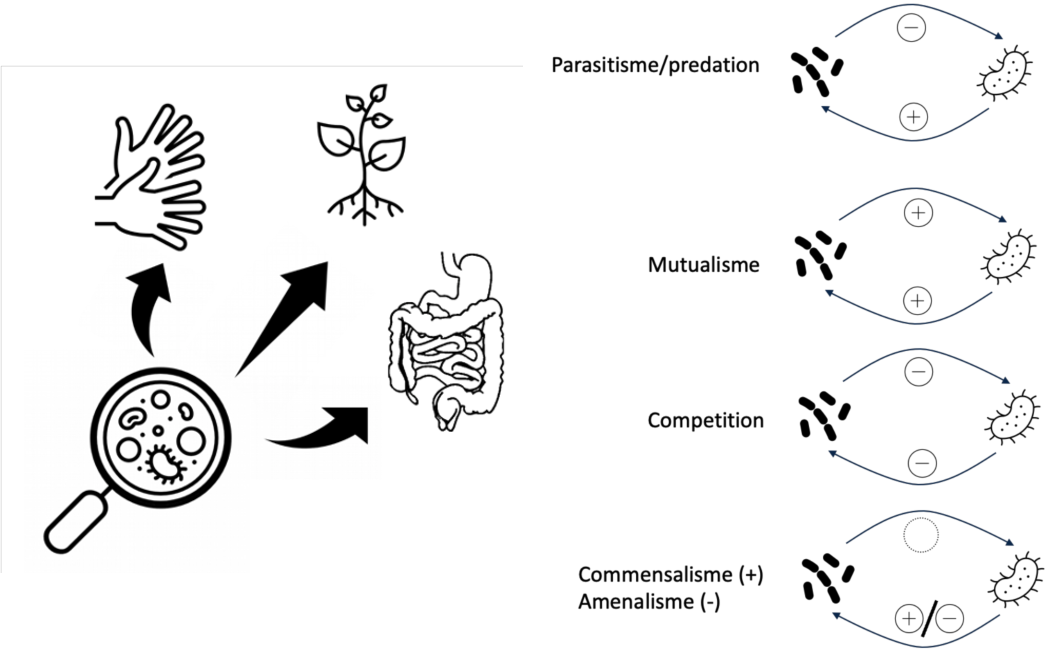
\includegraphics[width=\textwidth]{img/introduction/interaction.pdf}
    \caption{ \textbf{Présence de bactéries dans divers écosystèmes et illustrations des interactions bactériennes.} Un $+$  (respectivement $-$) signifie une interaction positive (respectivement négative). Un cercle en pointillé représente une interaction sans effet.}
    \label{fig:interaction}
\end{figure}
%
%%de trois méthodes hybrides. La première consiste à créer une approche hybride indépendant. TANGO et CoCoMiCo permettant tous deux la caractérisation de communautés bactérienne en utilisant deux approches différentes. Puis la création de 2 approches hybrides couplées : a) un système d'apprentissage entre CoCoMiCo et Tango. CoCoMiCo crible les métabolites d'intérêt à suivre dynamiquement dans TANGO et ce dernier communique sur la faisabilité de productibilité des métabolites via l'activation de réactions afin de contrainte le nombre de métabolites à suivre en dynamique. b) Etendre le programme MISCOTO en intégrant un solveur linéaire permettant de sélectionner des communautés basé sur les scores de coopération et compétition et en respectant des contraintes de tailles de communautés, de composition bactérienne et métabolites cibles.
%
%\begin{comment}
%
%\newpage
%\section{L'étude des écosystèmes microbiens}
%
%
%
%\subsection{Étude des interactions bactériennes}
%\subsubsection{Définition}
%A l'échelle de la communauté de bactéries, il existe des mécanismes sous-jacents permettant la communication entre le milieu nutritionnel et les bactéries et entre les bactéries entre elles, dénotées comme \textbf{interactions bactériennes}. Il existe plusieurs types d'interactions \citepp*{Faust2012} où chaque échange bacterien impact différemment les éspèces de la communauté. Dans \citepp*{Fons2000}, la conséquence de l'interaction bactérienne limite la croissance d'une autre autre, ou encore dans \citepp*{Kline2012}, une nouvelle éspèce apparait au sein de l'écosystème suite à une réaction immunitaire, affectant ainsi indirectement les autres membres de la communauté bacterienne.
%Les effets peuvent être déclinés de trois façon différentes : \textit{positive}, \textit{négative} ou \textit{neutre}. Plusieurs paramètres sont à prendre en compte lorsque l'on souhaite étiqueter des interactions bactériennes, comme par exemple, l'impact sur la croissance bactérienne ou bien sur le potentiel métabolique. En effet, une interaction permettant d'accroître la croissance et/ou la productibilité métabolique d'une espèce est considérée comme \textit{positive}, si au contraire, la croissance est réduite suite à la co-culture de deux espèce, on dit que l'interaction est \textit{négative}.  D'après \citepp{Faust2012} on parle de \textbf{coopération} lorsque l'interaction métabolique entre ces deux espèces est \textit{positive} pour les deux, le cas échéant, on parle de \textbf{commensalisme}. A l'inverse, la \textbf{compétition}, se traduit par une interaction métabolique \textit{négative} pour les deux espèces, et l'\textbf{aménalisme} que pour une des deux espèces. Enfin, lorsqu'à la fois une interaction \textit{positive} et \textit{négative} est observée pour une même paire d'espèce, on parle alors de \textbf{prédation} ou \textbf{parasitisme}.
%
%
%Toutes ces interactions bactériennes sont dépendantes de l'environnement nutritionnel. En effet, il existe des éléments du milieu que l'on peut qualifier de \textbf{limitant}, ou en \textbf{excès} conditionnant l'interaction bactérienne. On peut définir un substrat \textbf{limitant} comme une ressource qui deviendra non disponible à un moment donné dans le temps. A l'opposé, un métabolites en \textbf{excès} est une ressource qui sera toujours présente en quantité suffisante pour la communauté microbienne. En fonction de la nature \textbf{limitante} ou \textbf{excès} d'un nutriment, l'interaction bactérienne qui en découle, au sein d'une communauté donnée, en sera altérée. Ainsi, deux bactéries consommant un même nutriment limitant $l_A$ et un même nutriment en excès $e_B$ se traduira par une possible \textbf{compétition} seulement pour $l_A$.
%
%\subsubsection{Rôle dans un écosystème}
%Ces interactions bactériennes ont un rôle premier de maintien d'une population bactérienne au sein de l'écosystème \citepp{Braga2016}, et participe ainsi à son équilibre. Un rôle secondaire propre à chaque écosystème survient également. Dans \citepp{Cao2021}, un écosystème contrôlé composé de 3 bactéries participent à la production de composé aromatique lors de la production du fromage, ou encore, dans \citepp{Salas-Marina2011} où les interactions bactériennes permettent une meilleure résistance de la plante face à une infection. Une revue du rôle secondaire de ces interactions intrinsèque de l'écosystème est présentée dans \citepp{Braga2016}.\\
%
%Nous avons pu voir que l'étude des communautés bactériennes est centrée sur le mécanisme sous-jacent des interactions entre bactéries et se passe à l'échelle métabolique via l'echange de composés. Un moyen pertinent pour caractériser ces interactions consistent à étudier le métabolisme de chaque espèce. Le métabolisme regroupe toutes les réactions biochimiques portant les fonctions métaboliques associées. En étudiant le métabolisme de chaque espèce, on peut ainsi identifier le pouvoir métabolique, c'est à dire, l'ensemble des métabolites qui sont produit, l'ensemble des réactions activées ainsi que l'ensemble des métabolites qui sont consommés et déduire des interactions en communauté. De manière complémentaire, des données \textit{omiques}, caractérisant la structure, la fonction et même la dynamique d'un ou plusieurs organismes, sont nécessaires pour une analyse \textit{in silico} des communautés microbiennes.
%
% 
%\section{Données relatives à l'étude de communautés microbiennes : données \textit{Omiques}}
%Pour étudier les communautés bactérienne dans un environnement contrôlé et non contrôlé, le génome annoté de chaque individu est essentiel. En laboratoire, isoler les individus en culture pour extraire le génome puis le séquencer est une tâche commune. En revanche, dans le cas d'une communauté naturelle, composé de plusieurs centaines de bactéries et donc non cultivable en laboratoire, des données du type \textbf{métagénomiques} est alors requise. Un métagénome considère l'ensemble des génomes dans un biotope donné, toutes espèces confondues. Il existe ainsi deux méthodes prédominantes :  la métagénomique ciblée et la non ciblée \citepp{Perez-Cobas2020}.\\
%Dans le premier cas, un locus génomique d'intérêt est ciblé et synthétisé en quantité suffisante pour l'analyse. Un marqueur répondant aux contraintes d'universalité et de spécificité est alors choisi dans le but d'identifier les différents taxons. Concernant les bactéries, le marqueur de l'ADN ribosomique 16s est largement utilisé\citepp{Edgar2018} , l'espace de transcrit interne (ITS) est considéré comme un marqueur principal pour les champignons \citepp{Lucking2020}  et l'ADN ribosomique 18s pour les eukaryotes \maxime{REF}. Les séquences sont par la suite amplifiées et séquencées puis analysées. \\ 
%Au sein de la métagénomique non ciblée, le génome des espèces présentes dans le microbiome sont séquencées sans distinction taxonomique. L'ADN est extrait puis fragmenté en une centaine de paire de base et enfin amplifié avec diverses amorces dans le but de couvrir l'ensemble du matériel génétique contenu dans le microbiome. \\
%
%L'étude de communautés bactériennes peut se faire à différentes échelles d'analyse: le \textbf{transcriptome} et le \textbf{metabolome}. Le transcriptome correspond à la somme de tous les ARN messagers qui sont exprimés par les gènes d'un organismes. L'ensemble des méthodes permettant l'analyse qualitative et quantitative des ARN messagers s'appelle la \textbf{metatranscriptomique}. Tout comme la metagénomique, il existe différentes techonologies pour assembler les données transcriptomiques et les analyser \citepp{Lowe2017}. On retrouve d'une part les méthodes centrées sur l'expression d'individu avec les \textit{expressed sequence tag} ou EST ou encore, les analyses des expressions géniques en series ou (SAGE/CAGE). D'autre part, les méthodes focalisées sur l'ensemble des individus, telles que, le microarray \maxime{REF},  ou le RNA-SEQ, consistent en une combinaison de methode de haute génération séquençage et de méthodes computationnelles pour identifier les transcripts présents lors de l'extraction de l'arn \maxime{REF}.\\
%
%En plus de ces 2 types de données, l'ensemble des métabolites constituant un échantillon biologique, c'est à dire le \textbf{le metabolome}, associé aux méthodes d'analyses de données métabolomiques, identifient qualitativement ou quantitativement des potentiels bio-marqueurs responsables d'une maladie par exemple \citepp{Clish2015}. Il existe 3 grands types d'analyse en metabolomique : la (1) metabolomique ciblée, (2) le profilage et par (3) emprunte \citepp{Shulaev2006}. Brièvement, la méthode par la métabolomique ciblée consiste à mesurer précisément la concentration d'un ensemble de métabolites cibles et uniquement de cet ensemble. Celle par profilage mesure le niveau d'un ensemble de métabolites dans un échantillon, la mesure est pseudo-quantitative. Enfin, la dernière méthode permet d'identifier un motif caractérisant un instant du métabolisme dans un environnement particulier. \\
%
%\begin{figure}
%    \centering
%    \includegraphics{example-image-b}
%    \caption{Présentation des differentes données omiques en montrant le type d'information auquel on a accès (expression, ...). Ajouter dessus aussi la cible : pour les bactéries en culture, à la fois le genome individuel et de la métaG peut etre fait.}
%    \label{fig:my_label}
%\end{figure}
%
%Ces données omiques permettent une caractérisation à plusieurs échelles du fonctionnement d'une communauté de bactéries au sein d'un écosystème. Pour intégrer ces données omiques dans le but de caractériser une communauté bactérienne du point de vue des interactions, nous utilisons les réseaux métaboliques qui est une approximation du métabolisme. 
%
%\section{Défis de la modélisation microbienne}
%\maxime{récapituler les défis que l'on aura mis en avant dans le début de l'introduction plus un peu plus parler des défis de modélisation en générale.}
%
%Du point de vue d'un modélisateur ou d'une modélisatrice, le défi initial est la création d'un modèle avec le meilleur compromis entre précision des résulats, versatilité du modèle et temps de calcul en fonction des données en entrées. Dans le cas de la modélisation des écosystèmes microbiens, les mêmes problématiques sont retrouvées (voir chapitre \ref{ch:edla}), avec des modèles numériques permettant une analyse précise mais passant difficilement à l'échelle des communautés naturelles, et les modèles qualitatifs, sacrifiant la précision numériques au profil de méthodes criblant des communautés naturelles.\\
%
%
%Les défis liés à la modélisation du métabolisme microbiens sont multiples et sont dépendants du contexte biologique. En effet, cribler des communautés naturelles rapidement, avec une parfaite compréhension de l'ensemble du métabolisme de chaque individu au sein de la communauté permettant la prédiction de nouveau processus de régulation est utopique. Comme énoncé dans l'état de l'art numérique, la construction de modèles précis requiert une grande connaissance \textit{a priori} du système biologique (ODE) ou est limité par le temps de calcul d'une optimisation numérique. A l'inverse, les modèles discrets basés sur les graphs ou sur une optimisation combinatoire permet ce passage échelle, sont moins coûteux en temps mais leur précision est de l'ordre du qualitatif. Un compromis doit-être fait pour résoudre le criblage de grandes communauté bactérienne. Dans un premier temps, nous verrons l'apport d'un modèle numérique dans un environnement contrôlé. Le projet TANGO est composé de trois bactéries fromagères, \textit{L. lactis}, \textit{L. plantarum} et \textit{P. freudenreichii}. Nous avons développé une stratégie numérique basée sur le FBA pour l'intégration de multiples données omiques. Elle consiste en un raffinement des modèles FBA individuels par rapport à la connaissance biologique que l'on trouve dans la littérature ou apporté par l'expert ou l'experte biologique. A la suite, une calibration dynamique des modèles FBA par rapport aux données de croissance et à des données d'acides est faite. Enfin nous prédisons les croissances et les concentrations de chaque composé suivi dynamiquement en mettant en avant les contributions de chaque espèce. Une attention sera donnée aux interactions bactériennes mis en avant par cette stratégie. Dans un deuxième temps, le développement d'une approche par raisonnement applicable sur des écosystèmes naturels pour l'optimisation d'une communauté sera présenté. En effet, nous criblons des communautés créés aléatoirement provenant du sol, de la racine et feuille de la plante, et de l'intestin. A l'aide d'une approche de raisonnement, nous décrivons les communautés bactérienne sous forme d'un vocabulaire contrôlé. Ce dernier est alors utilisé pour estimer la coopération et la compétition dans les différents écosystèmes pour la suite, comparer des communautés de tailles équivalentes. Enfin, nous terminerons par l'élaboration de trois méthodes hybrides. La première consiste à créer une approche hybride indépendant. TANGO et CoCoMiCo permettant tous deux la caractérisation de communautés bactérienne en utilisant deux approches différentes. Puis la création de 2 approches hybrides couplées : a) un système d'apprentissage entre CoCoMiCo et Tango. CoCoMiCo crible les métabolites d'intérêt à suivre dynamiquement dans TANGO et ce dernier communique sur la faisabilité de productibilité des métabolites via l'activation de réactions afin de contrainte le nombre de métabolites à suivre en dynamique. b) Etendre le programme MISCOTO en intégrant un solveur linéaire permettant de sélectionner des communautés basé sur les scores de cooperation et competition et en respectant des contraintes de tailles de communautés, de composition bactérienne et métabolites cibles.
%
%\end{comment}
%
%\ifdefined\FromMain %
%\else % 
\end{document} %

